\documentclass[conference]{IEEEtran}
\IEEEoverridecommandlockouts
% The preceding line is only needed to identify funding in the first footnote. If that is unneeded, please comment it out.
\usepackage{cite}
\usepackage{amsmath,amssymb,amsfonts}
\usepackage{algorithmic}
\usepackage{textcomp}
\usepackage{xcolor}
\usepackage{enumitem}
\usepackage{calc}
\usepackage{graphicx}
\usepackage[colorlinks=true,urlcolor=blue,linkcolor=green]{hyperref}
\graphicspath{{images/}}

\usepackage{lipsum}

\def\BibTeX{{\rm B\kern-.05em{\sc i\kern-.025em b}\kern-.08em
    T\kern-.1667em\lower.7ex\hbox{E}\kern-.125emX}}
    
\begin{document}

\title{Medify -- A medication reminder Android App}

\author{\IEEEauthorblockN{Ekrem Emre}
\IEEEauthorblockA{\textit{HTWG Konstanz -- University of Applied Sciences, Germany} \\
\textit{Matriculation number: 302110} \\
ek741emr@htwg-konstanz.de}
}

\maketitle

\begin{abstract}
\lipsum[1][1-4]
\end{abstract}

\section{Introduction}

\section{Goal of the project}

\section{Requirement analysis}

\subsection{Personas}
To simulate users for this application, two personas were created, which represents the user types
that might us this application.

\subsubsection{First persona} \hfill
\begin{figure}[htbp]
	\centerline{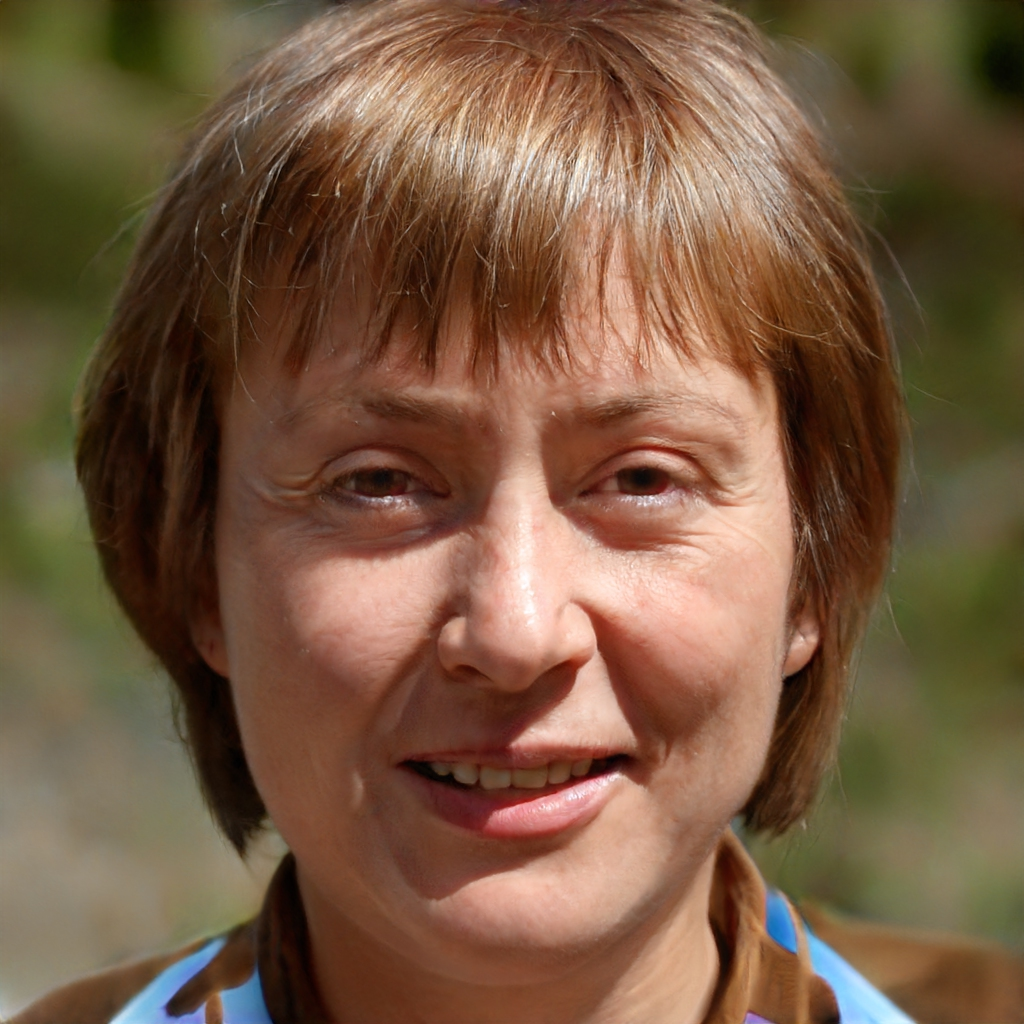
\includegraphics[width=.5\linewidth]{images/persona01.jpg}}
	\caption[Portrait of the persona Rosalyn Foster; Source taken from \cite{b1}]
	{\tabular[t]{@{}l@{}}Portrait of the persona Rosalyn Foster.\\ Source taken from \cite{b1}\endtabular}
	\label{fig:persona01}
\end{figure}

\begin{description}[labelwidth=\widthof{\bfseries Computer skills},leftmargin=.8cm,labelindent=.8cm]
	\item[Name] Rosalyn Foster
	\item[Age] 68
	\item[Marital status] Married
	\item[Occupation] Retiree
	\item[Computer skills] poor
\end{description}

\paragraph*{Key characteristics}
\begin{itemize}[leftmargin=1.25cm]
	\item Retiree, former tailor.
	\item Because of her advanced age, she got forgetful.
	\item Is regularly taking different medication, which she needs to be reminded of.
	\item Is concerned about her health, because she just became a grandparent and wants to spent as much time as possible with her grandchildren.
\end{itemize}

\paragraph*{Goals}
\begin{itemize}[leftmargin=1.25cm]
	\item Be healthy.
	\item Remember taking her medication regularly.
\end{itemize}

\paragraph*{User story}
As an older person, Rosalyn wants to be reminded to take her medicine, because she forgets them and wants to get healthy.

\subsubsection{Second persona} \hfill
\begin{figure}[htbp]
	\centerline{
\includegraphics[width=.5\linewidth]{images/persona02.jpg}}
	\caption[Portrait of the persona Christian Metz; Source taken from \cite{b1}]
	{\tabular[t]{@{}l@{}}Portrait of the persona Christian Metz.\\ Source taken from \cite{b1}\endtabular}
	\label{fig:persona02}
\end{figure}

\begin{description}[labelwidth=\widthof{\bfseries Computer skills},leftmargin=.8cm,labelindent=.8cm]
	\item[Name] Christian Metz
	\item[Age] 32
	\item[Marital status] Engaged
	\item[Occupation] Physiotherapist
	\item[Computer skills] strong
\end{description}

\paragraph*{Key characteristics}
\begin{itemize}[leftmargin=1.25cm]
	\item Working as a physiotherapist and doing a lot of sports, therefore is very healthy.
	\item He's a member in several sport clubs and a volunteer in the local animal shelter.
	\item His schedule is always pretty full and he's always on the go.
	\item He wants to increase his health by taking some vitamins, because he suspects he has some deficiencies.
\end{itemize}

\paragraph*{Goals}
\begin{itemize}[leftmargin=1.25cm]
	\item Be reminded, to take his vitamins.

\end{itemize}

\paragraph*{User story}
As a healthy person, Christian wants to be reminded to take his vitamins, because he's busy all day and not thinking of it and wants to stay healthy.

\subsection{Storyboards}

%\begin{figure*}
%	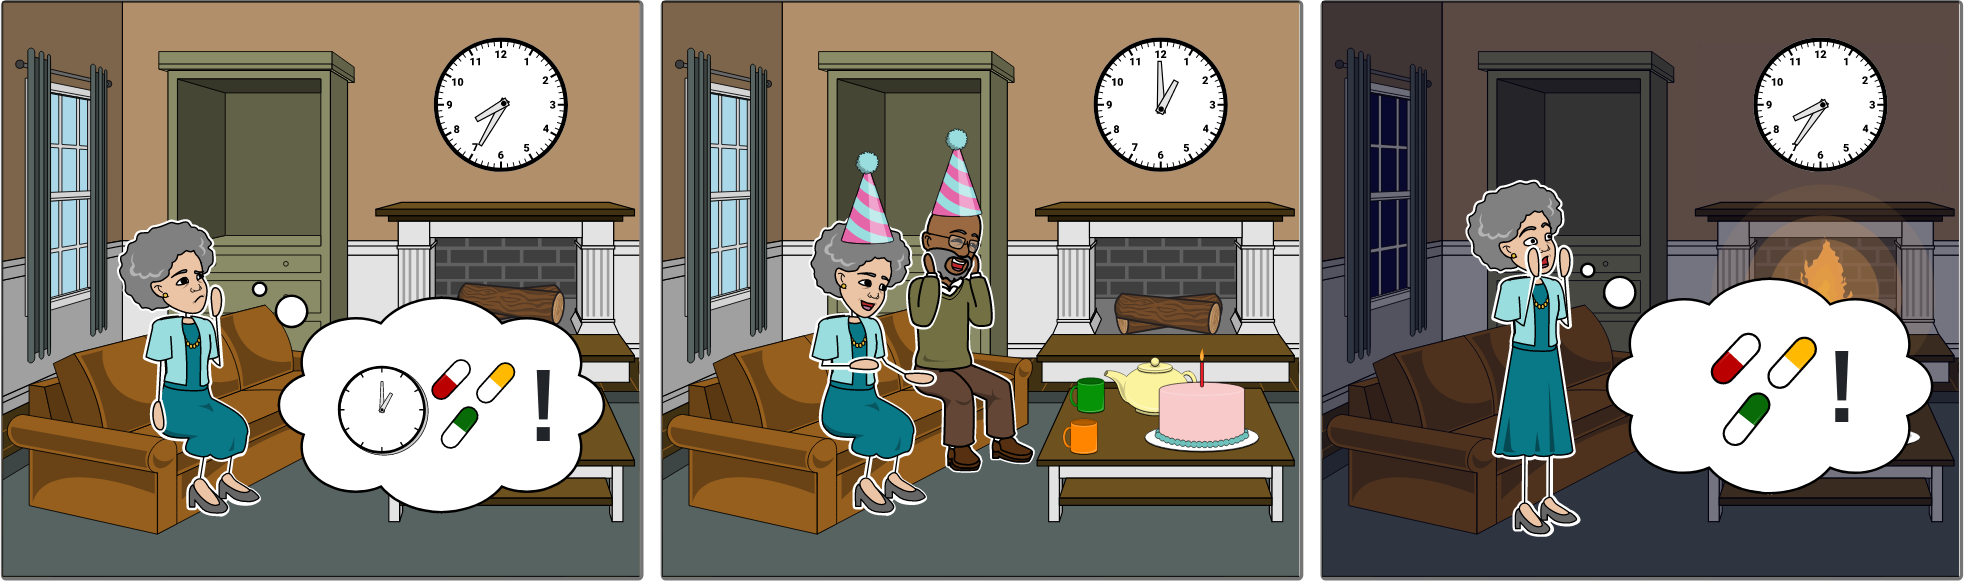
\includegraphics[width=\linewidth]{images/storyboard01.png}
%	\caption{TODO: this is the first storyboard.}
%	\label{fig:storyboard1}
%\end{figure*}
%
%\begin{figure*}
%	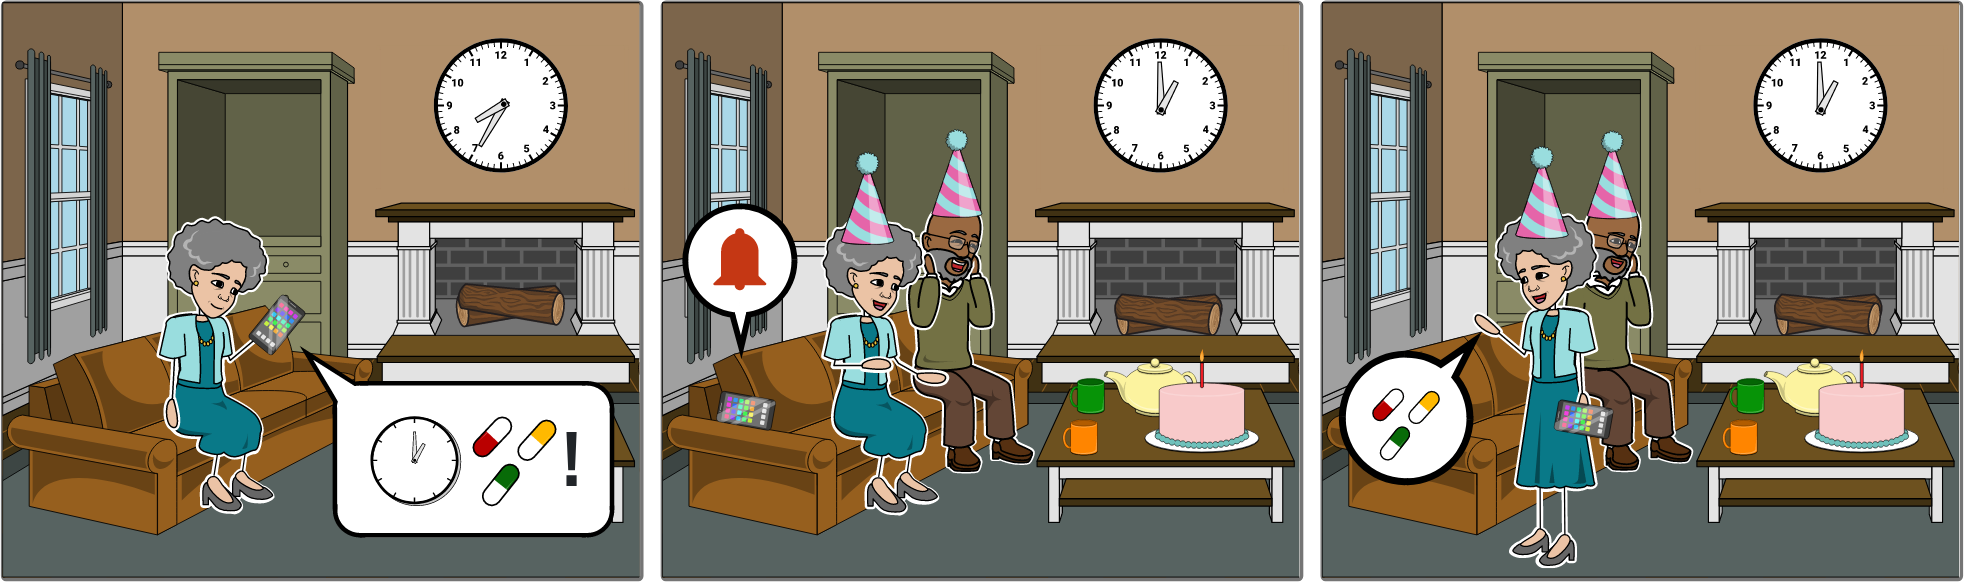
\includegraphics[width=\textwidth]{images/storyboard02.png}
%	\caption{TODO: this is the second storyboard.}
%	\label{fig:storyboard2}
%\end{figure*}


\section{Conceptual model of the solution}

\subsection{Entity relationship diagram}

\subsection{Activity diagram}

\subsection{Mockup}

\section{Design decisions}

\subsection{UML diagram}

\section{Results}

\section{Conclusion}


\begin{thebibliography}{00}	
	\bibitem{b1} P. Wang, ``This Person Does Not Exist,'' [Online] Available: \url{https://thispersondoesnotexist.com/} [Accessed Dec. 17, 2021].
\end{thebibliography}

\end{document}

